\section{Desarrollo y pruebas}
\label{secc:desarrollo y pruebas}
En este apartado se encontrarán las APIs usadas en Baldugenda, el uso de los dispositivos con un análisis de la elección de los mismos, un apartado referido al almacenamiento dentro de la base de datos de Baldugenda, se hablará sobre el aspecto de Backup dentro de la aplicación, y para finalizar este apartado, habrá una sección acerca de la interacción de los Baldusers con Baldugenda.
\subsection{Utilización de APIs}
\label{subsecc:Utilización de APIs}

En la aplicación de Baldugenda se han usado 3 APIs principalmente que son: la de Google Calendar, Google Drive y la de Splunk Mint.
El API de Google Calendar se ha usado para el manejo de los eventos de examen dentro del calendario de Google, y la creación y modificación de dichos eventos.
El API de Google Drive se ha usado para la realización del backup.
Y aunque Google nos proporciona medios para depurar la aplicación y ver qué tipos de dispositivos se la instalan, se ha decidido usar el API de Splunk Mint para esta función ya que ofrece información específica de los errores sin que el usuario que la está usando tenga que mandar nada.

\subsection{Dispositivos}
\label{subsecc:Dispositivos}

Uno de los requisitos que tenía que cumplir Baldugenda era el ser accesible a todo el que usara Android. La elección de la versión fue una labor difícil, porque hay muchos dispositivos con distintas versiones, por este motivo se optó por el mal menor y se fijó la versión de Android más baja posible que no diera problemas y que no quitara muchos usuarios.
La versión usada como mínimo en la aplicación fue la API 10-Gingerbread (2.3.3), según estadísticas de Google realizadas en mayo de 2015 la distribución de las versiones de Android es así \cite{dashboards}.


\begin{figure}
  \subfloat[Versiones de Android]{
   \label{f:Versiones de Android}
    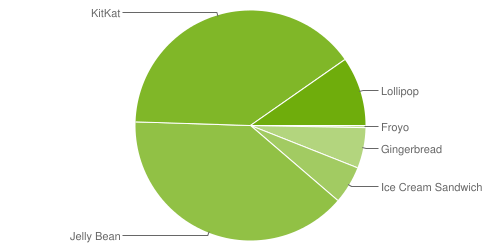
\includegraphics[width=0.5\textwidth]{figs/VersionesAndroid.png}}
  \subfloat[Tipos de pantalla]{
   \label{f:Tipos de pantalla}
    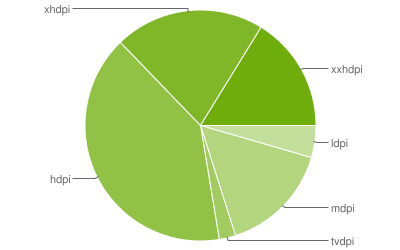
\includegraphics[width=0.38\textwidth]{figs/TiposPantalla.png}}
 \caption{Gráficos de dispositivos}
 \label{f:Gráficos de dispositivos}
\end{figure}

Aparte de la versión se tuvo que decidir para qué tipo de pantallas se lanzaría la aplicación, ya que optar por todas haría que la app pesara demasiado, por el hecho de incluir imágenes que se vieran bien en todas las pantallas sin la necesidad de redimensionar.
Se consultó el gráfico de pantallas de Google y se decidió dejar fuera la xxhdpi y a la ldpi y usar la mdpi,hdpi y xhdpi.


\subsection{Almacenamiento}
\label{subsecc:Almacenamiento}

Para el desarrollo de Baldugenda se optó por almacenar la información en ficheros sqlite que después el módulo de base de datos los leerá y los tratará para usarlos en las distintas actividades.
Durante toda la fase de implementación de Baldugenda, se ha ido modificando la BD hasta llegar a la versión tres, que es la que se está usando actualmente.
En cada una de las versiones se han ido añadiendo campos que pedían los Baldusers, y al crear una nueva versión de la BD se tuvo que ir actualizando las BDs, ya que hubo momentos en los que los Baldusers tenían versiones antiguas de la BD y no tenían que perder la información ya almacenada.
Estas actualizaciones se basaron en crear columnas nuevas en las tablas o llegar a recorrer las tablas enteras para organizar los datos.
Se crearon 3 tablas, una para las asignaturas, otra para los exámenes y la última para las notas de los exámenes.

Las tablas tienen las siguientes columnas:
\subsubsection{Asignaturas}
\label{subsubsecc:Asignaturas}

\textbf{Campo id incremental} clave primaria integer

\textbf{Nombre} campo único string, el nombre de la asignatura

\textbf{Enlaces}   un único string donde cada enlace que se presenta esta separado por “;”

\textbf{Evaluación} string que puede tener 2 valores Continua o Conjunta

\textbf{Nota} integer, será el valor máximo que se puede sacar en la asignatura

\subsubsection{Exámenes}
\label{subsubsecc:Exámenes}


\textbf{Campo id incremental} clave primaria integer

\textbf{Nombre} campo único string, el nombre del examen

\textbf{Asignatura} campo único string, el nombre de la asignatura

\textbf{Fecha} campo string, tendrá la fecha en formato DD/MM/AAAA

\textbf{Hora} campo string, tendrá la hora en formato HH:MM

\textbf{Tipo Guardado} campo string, puede tener 2 valores Ambos (si se ha podido crear el evento en Google Calendar) o Local  en caso contrario

\textbf{CalendarioId} campo string, tiene el id donde se ha generado el evento de Google Calendar

\textbf{EventoId} campo string, contiene el valor id del evento para ese examen

\textbf{CalendarioNombre} campo string, nombre del calendario donde se ha generado el evento de Google Calendar

\textbf{Descripción} campo string, descripción del examen

\subsubsection{Notas}
\label{subsubsecc:Notas}


\textbf{Campo id incremental} clave primaria integer

\textbf{Examen} campo único string, nombre del examen

\textbf{Asignatura} campo único string, nombre de la asignatura

\textbf{Nota} campo integer, nota sacada en el examen

\textbf{Nota\_Sobre} campo integer, nota máxima en el examen


Tanto en la tabla de exámenes, como en la de notas, se tuvo que especificar que la clave fuera un campo único con multivalor para que no se pudieran crear exámenes repetidos o duplicar notas.
El funcionamiento de la creación de la base de datos en Baldugenda se implementó de la siguiente manera: el sistema crea la versión uno de la BD, y el módulo de BD comprueba la versión disponible en el dispositivo. En el caso de que no haya una BD, el módulo de BD realizará las modificaciones para crear una BD versión tres. Si en el dispositivo se encuentra una versión anterior de la BD, solo realizará las modificaciones necesarias hasta alcanzar la versión tres.


\subsection{Backup}
\label{subsecc:Backup}

Para esta función de Backup se usó el API de Google Drive, el sistema le daba la opción al Balduser de exportar la base de datos a la carpeta que él quisiera de su Google Drive.
Para exportar, primero el módulo de Drive realizaba una conexión con el servicio de Google,éste a su vez comprueba que tiene los permisos necesarios para crear carpetas y ficheros, y una vez Google responde con una confirmación mediante el módulo de exportación, se accedía al Google Drive mediante una actividad que proporciona el propio API de Google Drive que muestra las carpetas el Drive, y el cual permite la posibilidad de crear nuevas carpetas.
Ya que la conexión era asíncrona se tuvo que separar la opción de seleccionar la carpeta donde el usuario subiría la base de datos, de la opción de volcar la base de datos a Google Drive. Si se realizaba junto, al intentar subir la BD, la aplicación se bloqueaba porque Google todavía no proporcionaba el id necesario para volcar la base de datos dentro de la carpeta creada.

A la hora de crear el fichero que se subía a Google Drive, el módulo de exportación realizaba una lectura de la base de datos de Baldugenda, después de haber leído toda la base de datos, esos se generaban en un formato de ByteArray para poder enviárselo a Google, Google generaría por medio del API un fichero que posteriormente lo almacenaría en Google Drive. Al hacer uso del API de Google Drive todos los funciones de creación y modificación dentro de Google Drive no se pudo ver cómo funcionaban por dentro. Tanto la creación, como la modificación de ficheros y carpetas, se realizó hasta el envío de los datos, a partir de ese momento Google se encargó de todo.

El sistema asignaba al fichero el nombre de la base de datos, y se le añadía la fecha y la hora en la que se había creado el fichero, para que el usuario pudiera escoger con facilidad ordenándolo por nombre.
Para importar la base de datos, lo único que tenía que hacer el usuario era seleccionar el fichero que se quería importar, y darle al botón de importar base de datos.
La lógica de negocio se encargará de descargar el fichero seleccionado de Google Drive, y creará un fichero nuevo en la ruta donde se encontraría la base de datos de Baldugenda, que en caso de que existiese un fichero en esa ruta, se borraría.

\subsection{Interacción con la app}
\label{subsecc:Interacción con la app}

Se realizaron pruebas a los Baldusers, y la mayoria realizaron las pruebas sin problemas, las respuestas que devolvieron eran que Baldugenda tenía una interfaz sencilla y de fácil manejo. Por este motivo, se puede suponer que el manejo de Baldugenda es sencillo, un ejemplo es que para acceder a la lista de asignaturas o a la lista de exámenes, sólo hace falta darle al icono del menú principal.
Aparte de este menú, que se basó en una serie de iconos con títulos que explica para qué es cada icono, se pueden ver las listas de asignaturas y de exámenes, cada lista tiene aspectos únicos que se han colocado para probar acciones dentro de una aplicación Android.
En la lista de asignaturas se puede encontrar un menú de búsqueda para que el usuario en el caso de que tenga muchas, al escribir el nombre de la asignatura en la caja de texto, le aparecería esa asignatura en la lista.

Aparte, se añadió la opción de la pulsación larga en cada asignatura para poder editarla o borrarla.
En la actividad de exámenes, se puede ver que la lista no es igual a la lista de asignaturas, se ha usado la clase ExpandableList para crear cajones donde debe ir la asignatura y los exámenes. Junto con el número de exámenes que hay dentro de la asignatura.
Se ha modificado el botón de atrás dentro de la actividad lista exámenes para que muestre un menú de navegación lateral para poder ir a cualquiera de las actividades mostradas. Se les preguntó a los Baldusers si les parecía buena idea el menú, y si era necesario incluirlo en cada una de las actividades, no respondieron al respecto. Por este motivo se decidió dejarlo únicamente en la actividad de lista exámenes para posibles mejoras.

\subsection{Android Studio}
\label{subsecc:androidStudio}

Para la implementación de Baldugenda se usó el IDE Android Studio, ya se había trabajado anteriormente con esta IDE, pero no se había implementado un proyecto como éste, ya que Baldugenda requería la implementacion de software realizado por terceros y para poder subirlo al Play Store se necesitaba firmar el apk que se generase. 

Android Studio ofrece ventajas frente a Eclipse, ya que desde hace pocos meses la comunidad de desarrolladores de Android le han dado más importancia al IDE de Android Studio y han dejado de lado a Eclipse. Eclipse al no ser un IDE exclusivo para Android, las funcionalidades que requerían las aplicaciones se solventaban mediante plugins, ocasionando fallos de compatibilidad de versiones.
\newpage
\subsection{Google Play Store}
\label{subsecc:Google Play Store}

Se uso el Play Store de Google para distribuir la aplicación a los usuarios que quisieran descargarsela. Para ello se tuvo que rellenar una serie de formularios y subir distintas capturas de la aplicación. Una vez subida al Play Store y activando la fase de producción el resultado es el siguiente.

\begin{figure}[H] 
  \begin{center} 
    \scalebox{0.4}{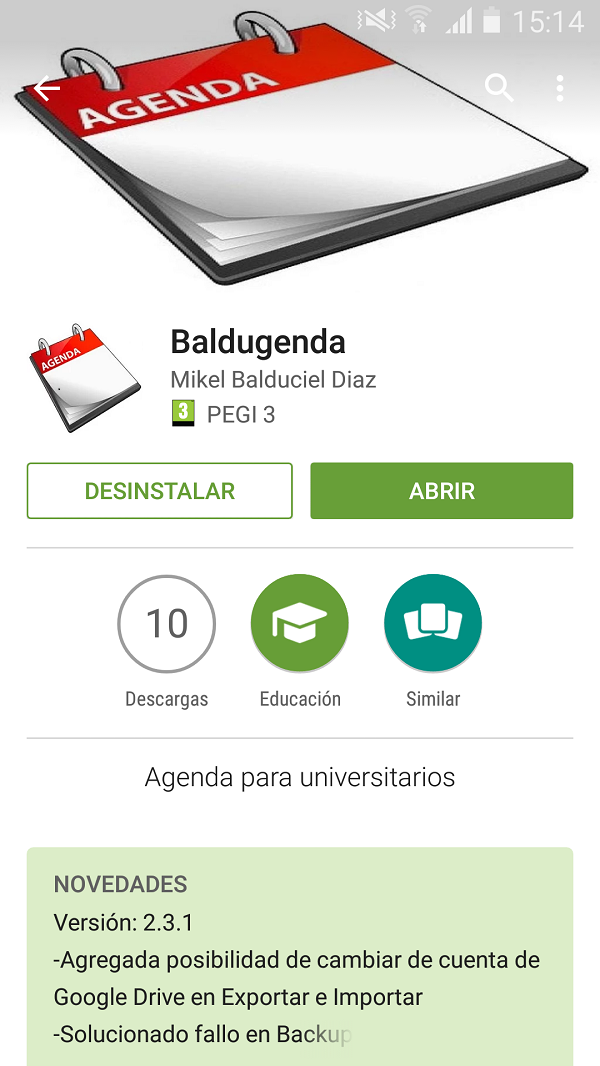
\includegraphics{figs/subida.png}} 
    \caption{Baldugenda en Play Store} 
    \label{fig:ModeloMVC} 
  \end{center} 
\end{figure}